\documentclass[9pt,conference]{IEEEtran}

\usepackage[hidelinks]{hyperref}
\usepackage{cite}
\usepackage{amsmath,amssymb,amsfonts}
\usepackage{algorithmic}
\usepackage{graphicx}
\usepackage{textcomp}
\usepackage{xcolor}
\usepackage{csquotes}
\usepackage{datetime}
\MakeOuterQuote{"}

% for nice tables
\usepackage{tabularx}
% \newcolumntype{b}{>{\centering\arraybackslash}X}
\newcolumntype{s}{>{\centering\arraybackslash\hsize=.5\hsize}X}
\newcommand{\heading}[1]{\multicolumn{1}{c}{#1}}
\renewcommand\tabularxcolumn[1]{m{#1}}% for vertical centering text in X column

\def\BibTeX{{\rm B\kern-.05em{\sc i\kern-.025em b}\kern-.08em
    T\kern-.1667em\lower.7ex\hbox{E}\kern-.125emX}}

% Quickly mark todos
\newcommand{\todo}[1]{\textcolor{red}{\small{TODO: #1}}}

\title{CS-523 SecretStroll Report\\\vspace*{20pt} \normalsize  \today{}}
\author{Furkan Karakaş, Pascal Andreas Schärli}
\author{\IEEEauthorblockN{Furkan Karakaş}
\IEEEauthorblockA{\textit{Department of computer and communication sciences} \\
\textit{École polytechnique fédérale de Lausanne}\\
Lausanne, Switzerland \\
\href{mailto:furkan.karakas@epfl.ch}{furkan.karakas@epfl.ch}}
\and
\IEEEauthorblockN{Pascal Andreas Schärli}
\IEEEauthorblockA{\textit{Department of computer science} \\
\textit{Eidgenössische Technische Hochschule Zürich}\\
Zurich, Switzerland \\
\href{mailto:pascscha@ethz.ch}{pascscha@ethz.ch}}
}

\begin{document}

\maketitle
\pagestyle{plain}

\begin{abstract}
In this report, we present the details of the second project SecretStroll of the PET course. The project consists of three parts. In Section \ref{sec:auth}, a secure, anonymous authentication mechanism is implemented by means of attribute-based credentials. In section \ref{sec:priv}, an attack is proposed to infer sensitive information about the users of the location-based service. Appropriate defense mechanisms are proposed to mitigate these attacks. Lastly, in Section \ref{sec:fingerprint}, the metadata in the network packets are used in a Tor network to perform a fingerprinting attack when a user sends a location request to the server.
\end{abstract}

\section{Introduction}

The aim of the project is to build a secure POI service where the client contacts a server to receive nearby points of interests in client's current location. The project consists of three parts. In the first part, a secure authentication mechanism is implemented. Instead of using a standard password and username-based authentication mechanism, we utilize the privacy-enhancing technology called \textit{attribute-based credentials} to authenticate the client to the server while still being able to hide a subset of his subscriptions. This way, the server does not store a hash of the password in the server-side and the server cannot run a hash-breaking algorithm to steal client's password. In the second part, we use the user trajectories to deduce sensitive information about the users. Next, we propose a defense mechanism to prevent the possible attack that we depicted here. Lastly, in the third part, we use a machine learning classifier that uses the meta-data in a Tor network to predict sensitive information about the users, i.e., what their subscriptions are.

\section{Attribute-based credential}
\label{sec:auth}
\subsection{PS-Signature}
In our attribute-based credential, we are working with an attribute map, which maps from the attribute names, e.g. \textit{"username"} to the values of these attributes, e.g. \textit{"Josh"}. We define the set of possible attributes for the issuer and then create a secret and public key over these attributes using an adapted version of the PS-Signature\cite{pointcheval2016short}, where instead of vectors we have maps from attribute names to their value within the PS signature. For example, instead of having a vector $(y_1,\ldots, y_r)$ we have a mapping $\{n_1 \rightarrow y_1, \ldots, n_r \rightarrow y_r\}$ that maps from each of the attribute names to its counterpart from the PS scheme. Indeed, this approach ensures that minimum information is revealed in each request. In the registration, the client reveals only the subscriptions that they want to subscribe. Furthermore, in the sign request step where the client requests a service from the server by revealing some of their attributes, the server can only observe the revealed attributes of the client and the server has no information about the other attributes which the client wanted to keep hidden from the server.

\subsection{Fiat-Shamir heuristic}
In our implementation of the Fiat-Shamir heuristic\cite{10.1007/3-540-47721-7_12}, we are given a multiplicative field with order $q$ and a set of bases $b$ and exponents $e$ with ${|b| = |e| = N}$. We want to show that we calculated ${C = \prod_{i=1}^{N}{b_i^{e_i}}}$ correctly without disclosing $e$. This is achieved by generating a random vector $n$ of size $N$ to calculate a commitment ${comm = \prod_{i=1}^{N}{b_i^{n_i}}}$. Using the public key $pk$, $C$ and $comm$, the challenge can be computed using the cryptographic hash function \textit{sha256} as follows: ${chal = sha256(C, pk, comm)}$. From there a response vector $r$ with $|r| = N$ and ${r_i = (n_i - e_i \cdot chal) \text{ mod } q}$ can be determined.

This proof can then be verified non-interactively, by at first calculating the challenge ${chal = sha256(C, pk, comm)}$ the same way as the proofing instance did. From there the commitment can be calculated using $b$ and $r$ as

$${comm' = C ^ {chal} \prod_{i=1}^N b_i ^ {r_i}}$$

The proof can then be verified by checking if $comm' = comm$.

\subsection{Registration}
We then start the attribute-based credential scheme with the user registration. The user creates an issue request with all of the subscriptions it would like to have as well as its username. This issue request contains a non-interactive Fiat-Shamir proof to prove that the issue request was calculated correctly. The server can then process the registration by verifying the proof that the issue request was calculated correctly and then signing the issue request. By our design choice, the client does not provide any of its own attribute values. All of the attributes are issued by the server. The server returns a blind signature using its secret key, which can then be used by the client to obtain a credential, consisting of a signature over all attribute names together with all attribute values. The client makes sure that the server issued correct subscriptions by checking the blind signature that the server sent to the client.

\subsection{Creating requests}
This credential can then be used by the client to sign a location request for a list of attributes. It creates a disclosure proof, disclosing all of the subscriptions for which it would like to get information from the server and hiding the other subscriptions as well as its username. The proof is again a non-interactive Fiat-Shamir proof and also incorporates an additional message which will contain the coordinates of the request. The server can then verify whether the disclosure proof is correct while also verifying the sent message. Through the disclosed attributes it can also check if the client has valid subscriptions for its request. 

\subsection{Test}
\subsubsection{Pointcheval-Sanders scheme}
We created two sets of secret and public keys $(sk_1, pk_1)$ and $(sk_2, pk_2)$ over a small set of attributes. Then a random message was signed with $sk_1$. The correct path is tested by assuring the signature verification succeeds with $pk_1$ and a failure path was tested by assuring the verification fails with $pk_2$.

\subsubsection{Fiat-Shamir heuristic}
The Fiat-Shamir heuristic was tested by generating random secret and public keys $(sk, pk)$ as well as a random base vector $b$ and exponent vector $e$ with $|b| = |e| = 100$. We create the proof over ${C = \prod_{i=1}^{100}b_i ^{e_i}}$. The correct path is tested by verifying the proof with the same $C$ and a failure path is tested by asserting the verification for $C' = C^2$ failure.

\subsubsection{ABC-Scheme}
We also tested a full run through utilizing all of our attribute-based credentials scheme methods. We define a list of attribute names and assign them random values. We chose which attributes to be user attributes, issuer attributes and which should be revealed or hidden. From there we follow all steps of the scheme until we obtain a credential. We assert that a normal disclosure proof on a random message verifies. Then we check two failure paths, one where the public key is different than the one used to obtain the credential and another one where the random message was changed in the verification step and make sure that these verifications fail.

\subsubsection{Stroll}
We tested the complete setup with the functions implemented in "\textit{stroll.py}". First, we ran the standard setup. We generate pk-sk pairs, client prepares for the registration, the server processes the registration request from client, client creates his credentials from the server's response, and client signs a location request with his credentials. In the standard setup, we verified that the server can indeed verify a correctly-generated signature from client. As a failure path, we verified that the server fails to verify a wrong signature from a bogus client.

As additional tests, we verified that client cannot subscribe for services which do not exist in the original subscriptions. We verified that client cannot reveal to the server the attributes which are not a subset of client's subscriptions. We verified that revealing no attributes to the server works correctly.

\subsection{Evaluation}
Performance of building blocks in our engine, namely key generation, issuance, signing, and verifying, is evaluated in terms of both communication and computational costs. Specifically, the effect of number of attributes is measured. The unit of computational costs is in milliseconds. The unit of communication costs is in number of bytes.

As the sample size, we use 100 iterations for computational costs and 1 iteration for communication costs because the communication size does not change between runs. We use \textit{"pytest-benchmark"}\cite{pytestbenchmark} software to perform our benchmark tests conveniently.

As the underlying hardware, we use Intel(R) Core(TM) i5-10210U CPU @ 1.60 GHz (8 CPUs), ~2.1 GHz and 8192MB RAM. The measurements are not directly conducted in the host operating system. Instead, we use Windows Subsystem for Linux (WSL) environment embedded into Windows 10.

It is apparent in \autoref{keygen} that the costs increase linearly with respect to the number of attributes for key generation. For the other functionalities, they seem to be somewhat linear but not exactly linear in \autoref{issuance}, \autoref{sign} and \autoref{verify}. We see that with few attributes, key generation is the quickest to complete. Although signing with few attributes takes more time than key generation, we observe that with increasing number of attributes, signing seems not to be badly affected by this unlike the others as with many attributes, signing takes the least time among others.

In \autoref{communication}, the communication costs of key generation and signing are zero since those operations do not require any data exchange. With issuance and verification, there seems to be a fixed cost $K$, and the overall cost increases linearly with the number of attributes $n$. This can be modeled as $cost=K+an$ for some $a>0$.

\begin{table}
\centering
\caption{Computational costs of keygen}
\label{keygen}
\begin{tabular}{cccccc}
\textbf{\#Attr.} & \textbf{Min} & \textbf{Median} & \textbf{Max} & \textbf{Mean} & \textbf{Std.} \\ \hline
5                &   2.7551           & 2.9552                &   5.4579           &   3.2168            & 0.6355              \\
10               & 4.8148             &  5.3348               & 7.6671             &  5.4428             & 0.4775              \\
20               & 8.5570             &  9.0765               & 11.9543             & 9.2608              & 0.6879              \\
50               & 19.8947             & 22.8428                & 29.6139             & 22.7490              &  2.1505             \\
100              &  39.3728            & 43.2605                & 57.7558             &  44.1520             &  3.6282             \\
500              &193.5952              & 209.5430                &250.7811              &212.6686               & 15.3274             
\end{tabular}
\end{table}

\begin{table}
\centering
\caption{Computational costs of issuance}
\label{issuance}
\begin{tabular}{cccccc}
\textbf{\#Attr.} & \textbf{Min} & \textbf{Median} & \textbf{Max} & \textbf{Mean} & \textbf{Std.} \\ \hline
5                & 10.1937             & 10.3903                &  15.8451            & 10.5896              & 0.7177              \\
10               & 14.8574             & 15.1841                & 23.5984             & 15.5657              &  1.1789             \\
20               & 23.9918             & 24.5973                & 34.1952             & 25.0160              &  1.2836             \\
50               & 52.4079             &  56.0415               &74.2870              &  58.2930             &  4.6360             \\
100              & 99.4769             & 102.7127                &131.3206              &  105.7491             &  7.2509             \\
500              & 478.0146             & 500.5404                & 708.9432             & 514.5282              & 34.7368             
\end{tabular}
\end{table}

\begin{table}
\centering
\caption{Computational costs of sign}
\label{sign}
\begin{tabular}{cccccc}
\textbf{\#Attr.} & \textbf{Min} & \textbf{Median} & \textbf{Max} & \textbf{Mean} & \textbf{Std.} \\ \hline
5                & 8.6187             &9.1978                 & 12.1171             & 9.5899              &   0.8686            \\
10               & 9.5018             & 9.9493                &  10.6755            & 9.9460              & 0.2177              \\
20               & 10.9892             &12.8955                &  15.6000            &   12.8808            &    1.2171           \\
50               &15.9726              &17.0995                 &21.6024              & 17.3606              & 1.2106              \\
100              & 23.9452             &24.9416                 &29.1585              &25.1153               & 0.8978              \\
500              & 91.0125             &95.8501                 &117.8290              & 97.7129              & 5.5549             
\end{tabular}
\end{table}

\begin{table}
\centering
\caption{Computational costs of verify}
\label{verify}
\begin{tabular}{cccccc}
\textbf{\#Attr.} & \textbf{Min} & \textbf{Median} & \textbf{Max} & \textbf{Mean} & \textbf{Std.} \\ \hline
5                &14.3352              &16.1703                 & 20.9394             &  16.2255             & 1.0479              \\
10               &21.5477              & 23.3880                &27.3911              &23.2753               & 1.1755              \\
20               & 34.8043             & 37.3630                &  42.3566            &   37.6724            & 1.7066              \\
50               & 74.0025             &  81.9556               & 95.0210             & 82.6141              &  5.7057             \\
100              & 140.4012             & 147.6422             & 172.0109             &149.5376               &  6.9097             \\
500              & 678.2764             &711.0836                 & 818.2849             & 717.7011              & 28.5575             
\end{tabular}
\end{table}

\begin{table}
\caption{Communication costs}
\centering
\label{communication}
\begin{tabular}{ccccc}
\textbf{\#Attr.} & \textbf{Keygen} & \textbf{Issuance} & \textbf{Sign} & \textbf{Verify} \\ \hline
5                & 0               & 5,448             & 0             & 3,408           \\
10               & 0               & 8,448             & 0             & 3,573           \\
20               & 0               & 14,478            & 0             & 3,913           \\
50               & 0               & 32,568            & 0             & 4,933           \\
100              & 0               & 62,718            & 0             & 6,633           \\
500              & 0               & 305,118           & 0             & 20,633         
\end{tabular}
\end{table}

\section{(De)Anonymization of User Trajectories}
\label{sec:priv}

We successfully implemented the anonymous credentials scheme, leading to an increase of privacy for our application. However, this privacy is impacted by the metadata sent along with the queries. In this stage of the application, the users reveal their IP addresses to the server whenever they make a query. In the following section, we assume that each user has exactly one, uniquely identifiable IP address. We will discuss the privacy implications in the case of an adversarial server.

\subsection{Privacy Evaluation}
With each query the server learns the IP address, current location of the user, the time of query and the POI (point-of-interest) type the user is querying for. We assume that there is a one-to-one correspondence between IP addresses and users. As we are assuming the server to be the adversary, it knows the position and POI type of any apartment block, villa, gym, dojo, office, laboratory and company building within the area of the queries. Although the queried locations always exactly matched an existing POI with the synthetic data set that we were given, our analysis also works for the more general case, where queries do not exactly lay on an existing POI.

In this analysis we aim to show how an adversarial server can try to determine home, workplace, possible hobbies and relationships from the given data and we try to deduce a social graph, showing the relations between the given users. We differentiate between the three categories home, work and sports and for each of those categories we would like to find the one POI which the user visited the most.

\subsubsection{Distance Score}
In the given data set the query locations match exactly the locations of the POIs. However in a real data set this is most likely not the case, which is why this approach calculates a score denoting how likely a user visited a place, depending on the distance of a user's query location and the given POI. This score is calculated by ${s_{dist}(d, q) = \frac{1}{(1+d/q)^2}}$ where $d$ is the distance between the query and the POI location in meters and $q$ is a parameter which configures how steep the curve is. This analysis worked with $q = 1$, however in a real-world scenario with more inaccuracy this parameter should likely be chosen bigger to have a less steep curve and more leniency towards inaccurate locations. An example of this function is shown in Figure~\ref{fig:distance-score}.

\begin{figure}
    \centering
    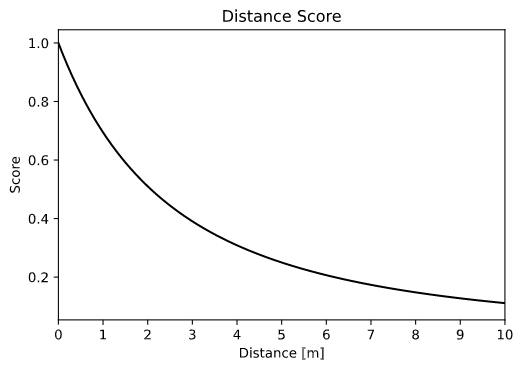
\includegraphics[width=0.55\linewidth]{images/distance-score.png}
    \caption{Distance score function for calculating the score of POI depending on its distance to the query. $q$ was chosen to be $5$ for this plot.}
    \label{fig:distance-score}
\end{figure}

\subsubsection{POI Categories}
Each category only regards a subset of all possible POI types. The category \textit{Home} regards \textit{apartment\_block} and \textit{villa}, \textit{Work} regards \textit{office}, \textit{laboratory} and \textit{company} and \textit{Sports} regards \textit{gym} and \textit{dojo}. As these categories are usually not equally relevant throughout the day, the POIs are further weighted for each category with a score that depends on the time of day and on the category:

$${s_{time}(t, l, m, n) = sin((x-12-l) \cdot \frac{\pi}{24})^n * (1-m) + m}$$

Here $t$ denotes the time of day in hours of the query and $l$, $n$, $m$ are configurable parameters to change the shape of the functions depending on the category. In our analysis we used the parameters from Table~\ref{tbl:time-score-params}, which resulted in scoring functions as shown in Figure~\ref{fig:time-score}. The scores from $s_dist$ and $s_time$ are multiplied together and summed up for each POI and category, leaving each POI with three scores for every user, symbolizing how likely this POI belongs to any of the three categories. For each category, the users are assigned the POI with the highest score in that category, leaving us with a guess of where the users live, where they work and where they do sports.

\begin{table}
\caption{Parameters for Time scoring}
\centering
\label{tbl:time-score-params}
\begin{tabular}{rccc}
\textbf{Type} & $l$ & $m$ & $n$ \\
\hline
Home & 0 & 0.25 & 2 \\
Work & 12 & 0 & 4 \\   
Sports & 16 & 0.25 & 20    
\end{tabular}
\end{table}

\begin{figure}
    \centering
    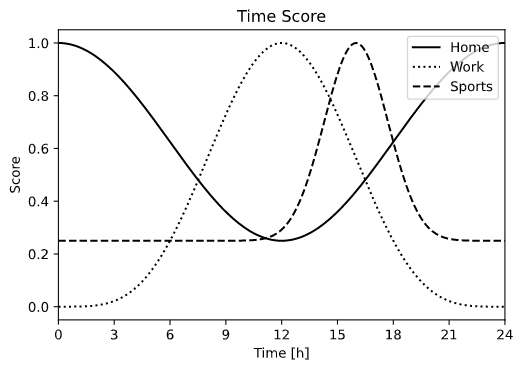
\includegraphics[width=0.75\linewidth]{images/time-scores.png}
    \caption{Time score function for POI categories for calculating the POI category score depending on the time of day of the query.}
    \label{fig:time-score}
\end{figure}

\subsubsection{Meetups}
Additionally to the categories mentioned above, our analysis also counts meetups between users. In this analysis, a user is assumed to be located at a POI, if $s_{dist} < 0.1$. If two users made a query at the same POI within 15 minutes, it is assumed that these users met.

\subsubsection{Findings}
Our analysis allows us to make a guess on where the users live, where they work and the number of estimated meetups indicates the strength of the relationship between two users. We cannot know for sure whether our guesses are correct or not, but the accuracy of the results was improved by the synthetic nature of the data set and the obtained relations between users seem plausible. These relations are summarized in Figure~\ref{fig:social-graph}.


\begin{figure}
    \centering
    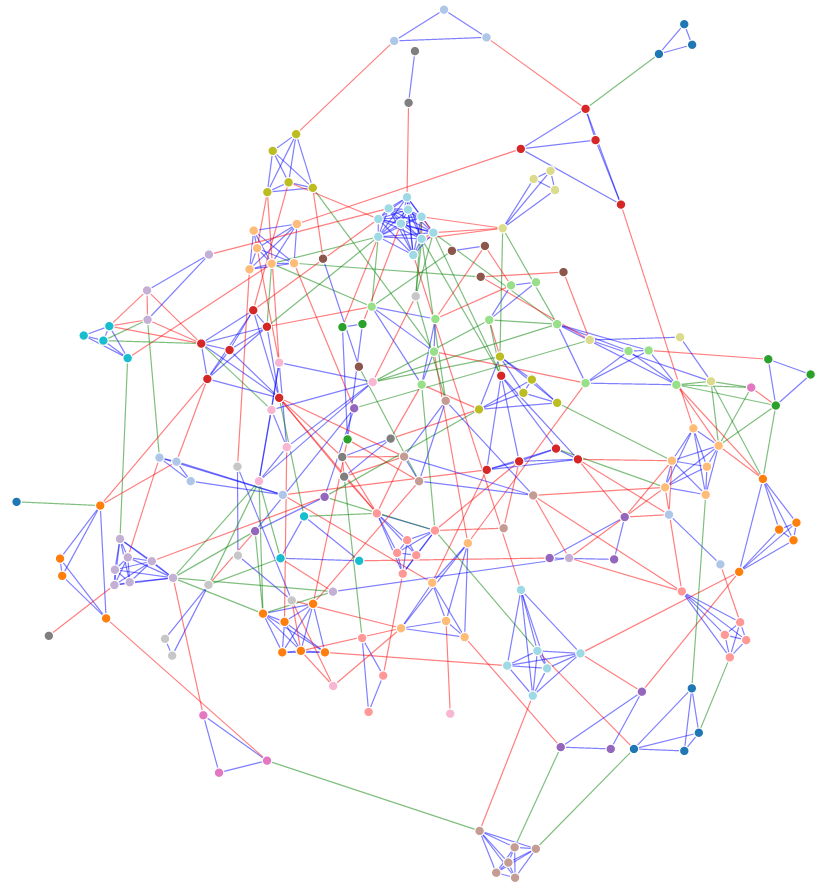
\includegraphics[width=0.5\linewidth]{images/social_graph.png}
    \caption{Social graph deduced from user attributes. Each node is a user and its color identifies its workplace. The locations of the nodes on the graph do not relate to their physical locations of their queries. The edge color indicates the relationship between the users, a blue edge means they work together, and a red edge means they live in the same house, otherwise the edge is green. Red and blue edges are only drawn if the users met more than 10 times for the red and blue edges or 15 times for the green edges during the recorded period.}
    \label{fig:social-graph}
\end{figure}


\subsection{Defences}

To avoid the problems described in the section above, we come up with a mechanism that is similar to the exponential mechanism in the differential privacy chapter. We assume that we have a \textit{passive} adversary in the server-side, i.e., the adversary can read the location request of the client. However, he cannot deny the service to the client, nor can he provide partial information about the points of interest in the requested location.

First, we note that we have fixed grids in the map. So, every grid will be represented by a fixed point inside of the grid, specifically the middle location in the grid. This is the trivial defense which has been mentioned in the project handout. We propose this from a utility perspective since it is desirable to be able to represent each grid with a single point in the form $(i,j)$, where $1 \leq i,j \leq 10$. Also, we note that there is no loss in sending the representative point of the grid since the user will receive exactly the same points of interest in either case.

Our mechanism works as follows. We define the Euclidean distance between two grid cells as

$$d(x,y) = \sqrt{(x_i-y_i)^2 + (x_j-y_j)^2}$$

where $1 \leq x_i,y_i,x_j,y_j \leq 10$. We define the utility score of a grid cell $y=(y_i,y_j)$ corresponding to a location request by the client in the grid $x=(x_i,x_j)$ as

$$u_x^{\epsilon}(y)=\frac{1}{(d(x,y)+1)^\epsilon}$$

where $\epsilon$ is the privacy parameter in our defense mechanism. We add one in the denominator to avoid division by zero when $x=y$. The purpose of the privacy parameter $\epsilon$ is that grids further away from the current grid of interest will receive smaller utility score as the privacy parameter grows. Hence, it will be more likely to choose the grid of interest with increasing $\epsilon$. So, in our model, a low epsilon corresponds to high privacy but low utility, and a high epsilon corresponds to low privacy but high utility, which is the utility-privacy trade-off in our model. Finally, we pick a grid cell $y$ with probability

$$P(y|x,\epsilon) = \frac{u_x^{\epsilon}(y)}{\sum_{m \in M} u_x^{\epsilon}(m)}$$

where denominator is the summation of all possible cells $m$ in the map $M$.

\begin{figure}
    \centering
    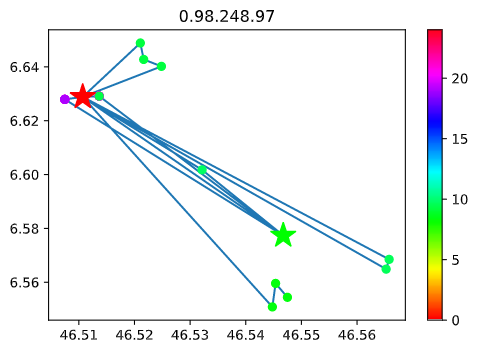
\includegraphics[width=0.5\linewidth]{images/0.98.248.87_insecure.png}
    \caption{Mobility of the user corresponding to the IP address 0.98.248.97 in the week. The color legend is the time of day from 0 to 23.}
    \label{fig:insecure}
\end{figure}

\begin{figure}
    \centering
    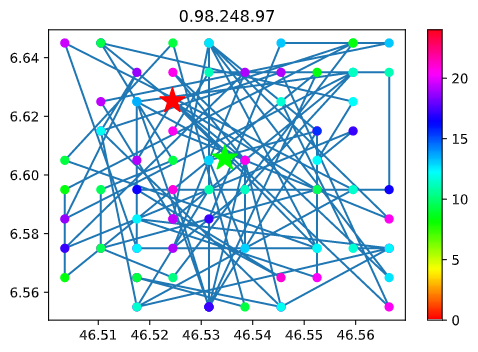
\includegraphics[width=0.5\linewidth]{images/0.98.248.87_secure.png}
    \caption{The same mobility data after the defense mechanism has been applied. The color legend is the time of day from 0 to 23.}
    \label{fig:secure}
\end{figure}

In Figure \ref{fig:insecure}, the attack performed on the user with IP address 0.98.248.97 is shown. In the figure, we show two stars with colors red and green, which show the most frequent places the user is in during the night and day times. They can correspond to user's home and work places. After applying the defense mechanism to the \texttt{queries.csv} file, we obtain the user trajectories depicted in Figure \ref{fig:secure}. We note that after applying the defense mechanism, the user trajectories are scattered across the map, and the new estimated home and work places are not the same as the one found in Figure \ref{fig:insecure}. With this new setup, the attacker needs to work more and harder to retrieve the sensitive information for the users.

As additional, not easily quantifiable privacy mechanisms, we propose

\begin{itemize}
    \item \textit{client-side caching}, where the user stores a cache of the history of his requests in his smart phone. This way, the location service will not be contacted frequently and the chance of a successful attack will diminish significantly. In return, the utility in terms of new points of interests in the map and memory usage in the smart phone will diminish,
    \item \textit{sending bogus requests}, where the client requests additional locations on top of the location of true interest. If the user requests many locations, he gets more privacy but he will also get less utility since the app will drain more battery power. As the extreme case, the client requests all POIs from the service provider. In this case, the server has no means to determine what user's true request is. On the other hand, there will be huge communication overhead and the battery consumption of the app will be high.
\end{itemize}

\section{Cell Fingerprinting via Network Traffic Analysis}
\label{sec:fingerprint}

\subsection{Implementation details}
\subsubsection{Data collection}
The data used for fingerprinting the network traffic was collected as \textit{PCAP} files, using \texttt{tcpdump}\cite{tcpdump}. The traffic could have been captured from the host machine, but as this would have required to filter for the traffic from the client container, we chose to capture the traffic directly from within the client's container, as this inherently only captures traffic going from the client to the internet. Traffic filtering was not necessary, as in our setup all traffic was caused by our client program communicating with the Tor entry node. The capturing process was automated and limited the packet capturing to exactly the traffic caused by a single query, which was used to collect traffic of around 50 samples for each possible queried grid number.
\subsubsection{Features extraction}
The choice of features greatly impacts the performance of the classifier. The traffic captured in the previous step were in \textit{PCAP} format, which entails a lot of unnecessary metadata. From these captures we parsed the individual packets, which were filtered to only contain packets using the \textit{IP} protocol, containing a body with \textit{Raw} data, where exactly one of the sender or recevier are within the local network and which were not of size 54. The latter is to filter out \textit{TCP ACK} packets, as suggested by Andriy Panchenko et al.\cite{panchenko2011website}. These filtered packets were then used to obtain the following feature sets:
\begin{itemize}
    \item \textit{Basic Counts}: The total number and size of all packets, considering incoming and outgoing packets separately.
    \item \textit{Packet Sizes}: A list of all packet sizes across the capture.
    \item \textit{Packet Size Accumulations}: The packet lengths accumulated such that each entry holds the sizes of all packets received up to that point. An example of such an accumulation can be seen in Figure~\ref{fig:features}.
    \item \textit{Incoming Packet Accumulations}: The same as packet accumulations but filtered to only regard packet sizes of incoming packets.
    \item \textit{Outgoing Packet Accumulations}: The same as packet accumulations but filtered to only regard packet sizes of outgoing packets.
    \item \textit{Size Histogram}: A histogram, with the buckets representing the accumulated packet sizes, filled by the amount of time a capture was stagnating at this accumulated size. An example of such an accumulation can be seen in Figure~\ref{fig:features}.
\end{itemize}

Additionally the feature sets \textit{Size Markers}, \textit{Number Markers}, \textit{Occurring Incoming Packet Sizes}, \textit{Occurring Outgoing Packet Sizes}, \textit{Percentage Incoming Packets} and \textit{Number Of Packets} that are suggested by Andriy Panchenko et al.\cite{panchenko2011website} were also evaluated. The length of some of these feature sets are dependent on the length of their packet capture, which varies across the different queries and measurements, so these features were zero-padded in order to ensure each feature vector has the same length.

\subsubsection{Classifier}
The classifier of the provided code skeleton was not changed. The classification was conducted with a random forest classifier on a subset of the above mentioned features. To evaluate the performance of the feature sets, all possible combinations of up to three feature sets were evaluated with 10-fold cross validation.

\begin{figure}
    \centering
    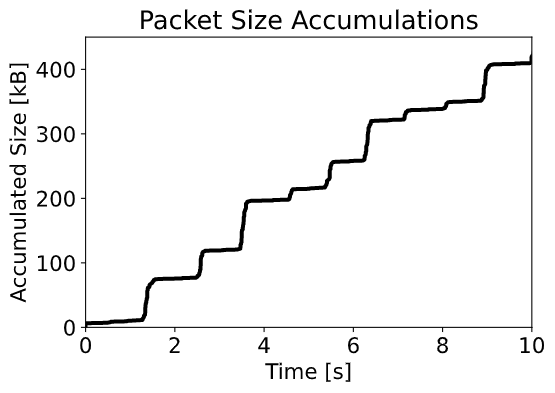
\includegraphics[width=0.45\linewidth]{images/size_accums.png}
    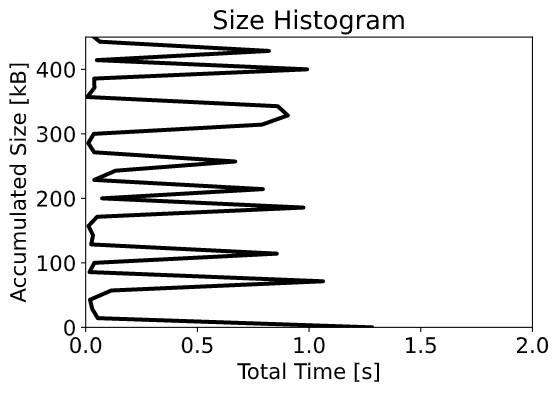
\includegraphics[width=0.45\linewidth]{images/histogram.png}
    \caption{Left: Packet size accumulation for a sample traffic capture. Right: Histogram showing for how long each accumulated size was present.}
    \label{fig:features}
\end{figure}

\subsection{Evaluation}
Not all feature sets had the same effectiveness. The feature sets described by Andriy Panchenko et al.\cite{panchenko2011website} achieved an accuracy of around 65\%, which is similar to the accuracies described in their report, despite using another classifier than they suggest and our data set not being \textit{HTTP} web traffic. The best performances were achieved using our \textit{Size Histogram} feature set, which manages to achieve the best results, achieving a maximal accuracy of around 95\%. Table~\ref{table:top_5} shows the 5 best performing feature set combinations, which all included our our \textit{Size Histogram} feature set. In fact, any feature set combination that included this \textit{Size Histogram} outperformed all of the combinations which did not use this \textit{Size Histogram}. Table~\ref{table:top_5_no_hist} shows how the best feature set combination that does not contain the \textit{Size Histogram} achieves an accuracy of around 71\%.

\begin{table}
\caption{Best feature set combinations}
\centering
\label{table:top_5}
\begin{tabularx}{\linewidth}{cccs}
\textbf{Rank} & \textbf{Accuracy} & \textbf{Std. dev.} & \textbf{Feature sets} \\ \hline
1.               & 0.95833               & 0.00859             & \textit{Size Histogram}, \textit{Basic Counts}  \\
2.               & 0.95753               & 0.00693             & \textit{Size Histogram}, \textit{Basic Counts}, \textit{Number of Packets}          \\
3.               & 0.95753               & 0.00900             & \textit{Size Histogram}, \textit{Basic Counts}, \textit{Percentage Incoming Packets}           \\
4.               & 0.95712               & 0.00859             & \textit{Size Histogram}, \textit{Percentage Incoming Packets}           \\
5.               & 0.95711               & 0.00824             & \textit{Size Histogram} \\
\end{tabularx}
\end{table}

\begin{table}
\caption{Best feature set combinations without Size Histogram}
\centering
\label{table:top_5_no_hist}
\begin{tabularx}{\linewidth}{cccs}
\textbf{Rank} & \textbf{Accuracy} & \textbf{Std. dev.} & \textbf{Feature sets} \\ \hline
68.               & 0.71339               & 0.01248 & \textit{Packet Size Accumulations}, \textit{Basic Counts}, \textit{Percentage Incoming Packets} \\
69.               & 0.71157               & 0.01273 & \textit{Packet Size Accumulations}, \textit{Basic Counts}, \textit{Occurring Outgoing Packet Sizes} \\
70.               & 0.70753               & 0.01730 & \textit{Packet Size Accumulations}, \textit{Basic Counts} \\
71.               & 0.70753               & 0.01539 & \textit{Packet Size Accumulations}, \textit{Basic Counts}, \textit{Number of Packets} \\
72.               & 0.70632               & 0.01480 & \textit{Incoming Packet Accumulations} \\
\end{tabularx}
\end{table}


\subsection{Discussion and Countermeasures}
We got the best accuracy of $95.83 \pm{0.86} \%$ with the features \textit{Size Histogram} and \textit{Basic Counts}. We see from Table~\ref{table:top_5} that the feature set \textit{Size Histogram} alone has has a performance of $95.71\%$ accuracy. In our attack, we exploited the fact that the server sends the data for POI not together but in distinct intervals, which is a strong indicator for our random forest classifier. We have a couple of counter-measures against this attack.

\subsubsection{Avoid stairs}
In the captured PCAP file, an attacker can observe clear stairs where there is little-to-no data transmission in one phase and a surge of network activity in another. To avoid this attack, we propose that the server should accumulate every POI in the back-end and it should respond back once every POI is retrieved. The utility trade-off for this privacy mechanism is that the user will have to wait until the end of the transmission for all packets to arrive, and only after that they will be able to view the relevant POI in the region.

\subsubsection{Padding}
The attacker used the fact that not every grid cell contains the same number of POIs. To mitigate this problem, we propose to send the same size of data every time the user issues a request by padding the server's response with redundancy, where this size could be proportional to the maximum number of POIs in the grid cells. Again, there is a utility-privacy trade-off in this protection that we propose, which is increasing the network traffic and data usage.



\bibliographystyle{IEEEtran}
\bibliography{bib}
\end{document}
